%%%%%%%%%%%%%%%%%%%%%%%%%%%%%% -*- Mode: Latex -*- %%%%%%%%%%%%%%%%%%%%%%%%%%%%
%% nsf.tex         : 2009 CPATH Proposal
%% Author          : Philip Johnson
%% Created On      : Tue Mar 31 11:16:58 2009
%% Last Modified By: Philip Johnson
%% Last Modified On: Sat Apr 25 08:49:23 2009
%%%%%%%%%%%%%%%%%%%%%%%%%%%%%%%%%%%%%%%%%%%%%%%%%%%%%%%%%%%%%%%%%%%%%%%%%%%%%%%
%%   Copyright (C) 2009 
%%%%%%%%%%%%%%%%%%%%%%%%%%%%%%%%%%%%%%%%%%%%%%%%%%%%%%%%%%%%%%%%%%%%%%%%%%%%%%%
%% 
 
\documentclass{proposalnsf}
\usepackage[final]{graphicx}

% NSF proposal generation template style file.
% based on latex stylefiles  written by Stefan Llewellyn Smith and
% Sarah Gille, with contributions from other collaborators.

\renewcommand{\refname}{\centerline{References cited}}
\newcommand{\eCT}{{\it e}CT}

% Fix things so that figures tend to stay away from the last page. 
\renewcommand{\topfraction}{0.85}
\renewcommand{\textfraction}{0.1}
\renewcommand{\floatpagefraction}{0.75}

% this handles hanging indents for publications
\def\rrr#1\\{\par
\medskip\hbox{\vbox{\parindent=2em\hsize=6.12in
\hangindent=4em\hangafter=1#1}}}

\def\baselinestretch{1}

\begin{document}

%%%%%%%%%%%%%%%%%%%%%%%%%%%%%%% -*- Mode: Latex -*- %%%%%%%%%%%%%%%%%%%%%%%%%%%%
%% summary.tex -- 
%% Author          : Philip Johnson
%% Created On      : Tue Mar 31 11:42:10 2009
%% Last Modified By: Philip Johnson
%% Last Modified On: Wed Apr 22 11:50:12 2009
%% RCS: $Id$
%%%%%%%%%%%%%%%%%%%%%%%%%%%%%%%%%%%%%%%%%%%%%%%%%%%%%%%%%%%%%%%%%%%%%%%%%%%%%%%
%%   Copyright (C) 2009 
%%%%%%%%%%%%%%%%%%%%%%%%%%%%%%%%%%%%%%%%%%%%%%%%%%%%%%%%%%%%%%%%%%%%%%%%%%%%%%%
%% 

\section*{Project Summary}
\renewcommand{\thepage} {A--\arabic{page}}

%% {\em The proposal must contain a summary of the proposed activity suitable for
%% publication, not more than one page in length. It should not be an abstract
%% of the proposal, but rather a self-contained description of the activity
%% that would result if the proposal were funded. The summary should be
%% written in the third person and include a statement of objectives and
%% methods to be employed. It must clearly address in separate statements
%% (within the one-page summary):

%% (1) the intellectual merit of the proposed activity; and

%% (2)the broader impacts resulting from the proposed activity. 

%% It should be informative to other persons working in the same or related
%% fields and, insofar as possible, understandable to a scientifically or
%% technically literate lay reader. Proposals that do not separately address
%% both merit review criteria within the one-page Project Summary will be
%% returned without review.
%% }


\noindent {\bf Overview.}  The vision of this proposal is to develop and
institutionalize a new approach to computational thinking where abstraction
and automation combine to transform the use of {\em empirical thinking} in
software development.  We call this approach ``empirical computational
thinking'', or \eCT.  The goal of this research is to explore, evaluate, and institutionalize
techniques and technologies for \eCT, building upon research and education
by ourselves and others in empirically-based software development.

\medskip

\noindent {\bf Intellectual Merit.}  First, this project will create and
institutionalize the notion of empirical computational thinking as a useful
component for programming courses. Second, this project will create a new
community of research and practice around the unifying concept of empirical
computational thinking.  Third, this project will generate a new mechanism
for evaluating initiatives in empirical computational thinking: the Common
\eCT\ Evaluation Framework. Fourth, this project will lead to significantly
increased use of \eCT\ initiatives in computer science curriculum. Fifth,
this project will generate new empirical data sets regarding software
development activities in a classroom setting.


\medskip 

\noindent{\bf Broader Impacts.}  First, this project will serve
underrepresented populations, as the University of Hawaii is an EPSCOR
state. Approximately 84\% of undergraduates at the University of Hawaii are
minorities, and the computer science students exemplify this diversity.
Second, the software engineering curriculum at the University of Hawaii is
well-regarded within the local high tech community, and many of its
graduates have gone on to leadership positions. A successful \eCT\
initiative could thus be transformative beyond the college and into the
local community.  Third, this project supports the NSF goal of fostering
integration of research and education.  The research outcomes regarding
\eCT\ will impact directly on classroom practice.  Fourth, this project
creates a basis for future directions including expansion of \eCT\ concepts
into non-CS disciplines such as English or Architecture, and the
application of \eCT\ to scientific, evidence-based thinking.

%%%%%%%%%%%%%%%%%%%%%%%%%%%%%% -*- Mode: Latex -*- %%%%%%%%%%%%%%%%%%%%%%%%%%%%
%% project.tex -- 
%% Author          : Philip Johnson
%% Created On      : Tue Mar 31 11:44:58 2009
%% Last Modified By: Philip Johnson
%% Last Modified On: Fri Apr 24 13:47:06 2009
%% RCS: $Id$
%%%%%%%%%%%%%%%%%%%%%%%%%%%%%%%%%%%%%%%%%%%%%%%%%%%%%%%%%%%%%%%%%%%%%%%%%%%%%%%
%%   Copyright (C) 2009 
%%%%%%%%%%%%%%%%%%%%%%%%%%%%%%%%%%%%%%%%%%%%%%%%%%%%%%%%%%%%%%%%%%%%%%%%%%%%%%%
%% 

\pagenumbering{arabic}
\renewcommand{\thepage} {C--\arabic{page}}

\renewcommand{\thesection} {C.\arabic{section}}
\setcounter{section}{0}

\section{Project Description}

\subsection{Project Vision, Goals, Objectives, and Outcomes}

%% {\em Section requirements: Describe the CT-centric vision, goals,
%% objectives, and anticipated outcomes of the proposed project. Clearly
%% indicate how they will contribute to realization of the three CPATH program
%% goals: (1) contribute to the development of a globally competitive
%% U.S. workforce with CT competencies essential to U.S. leadership in the
%% global innovation enterprise; (2) increase the number of students
%% developing CT competencies by infusing CT learning opportunities into
%% undergraduate education in the core computing - computer and information
%% science and engineering - disciplines, and in other fields of study; and,
%% (3) demonstrate transformative CT-focused undergraduate education models
%% that are replicable across a variety of institutions.

%% Evaluation criteria: Assess the potential of the proposed project and the
%% likelihood that it will contribute in significant ways to realization of
%% the CPATH program goals.
%% }
%% \bigskip

Jeannette Wing has written, ``Computational thinking involves solving
problems, designing systems, and understanding human behavior, by drawing
on the concepts fundamental to computer science'' \citep{Wing06}.  In her
presentation ``Computational Thinking and Thinking About Computation'',
Wing refines her view of these fundamental computer science concepts in terms of 
the ``Two As'': Abstraction and Automation.  Activities
related to the first ``A'' include: choosing the right abstractions, operating
at multiple levels of abstraction, and defining relationships between
abstractions.  Activities related to the second ``A'' involve mechanizing the
first A via precise notations and models.  In essence, automation amplifies
the power of abstraction.  Computational thinking, from this perspective,
involves the correct choice of abstraction combined with the correct choice
of automation.

The vision of this proposal is to develop and institutionalize a new
approach to computational thinking where abstraction and automation combine
to transform the use of {\em empirical thinking} in software development.
We call this approach ``empirical computational thinking'', or \eCT.

To introduce our approach, we must first address what is meant by
empirical thinking.  The term ``empirical'' is variously defined as
``derived from experiment and observation rather than theory''; ``evidence
or consequences observable by the senses''; and ``capable of being verified
or disproved by observation or experiment.''

Given these definitions, it is clear that some degree of empirical thinking
is already commonplace in software development.  For example, beginning
programmers use empirical thinking when they ``observe'' the output of the
compiler to learn how to write syntactically correct programs.  Beginners
also tend to make extensive use of ``experimentation'': they execute their
program with example data, compare the actual behavior to what they expect,
then make modifications until the observed behavior matches their
expectations.

These examples of empirical thinking, while typical for beginning
programmers, do not scale well because they lack both abstraction and
automation. Thus, they fail to constitute the kind of computational
thinking of interest to the CPATH program, and they fail as well to be
\eCT.

One would hope that as students progress into more advanced software
development courses, the curriculum would scale in at least two
ways. First, the complexity, size, and number of people involved in a
software development project would scale upwards.  Second, the level of
abstraction and automation in their empirical thinking would scale
commensurately. Unfortunately, while advanced software development courses
certainly require students to develop significantly more sophisticated
systems than their introductory counterparts, the use of empirical thinking
remains mostly non-abstract and non-automated.  The principle computational
support for advanced programming classes is an integrated development
environment such as Eclipse or Visual Studio. While this is a significant
advance over vanilla text editors, such IDEs provide relatively little in
the way of abstraction or automation for empirical thinking about the
products and processes of software development.

Supporting abstraction in empirical thinking for software development
generally means creating quantitative models for important development
concepts.  For example, test quality is an important concept that is
commonly emphasized in advanced software development courses.  One
quantitative model for test quality is line-level test coverage, which is
generally expressed as the percentage of source lines of code in the
software exercised by the test cases.  Another important concept is
complexity, and quantitative models such as afferent and efferent coupling
or cyclomatic complexity provide abstract, empirical representations for
this concept. Some aspects of design quality can be observed through tools
that, for example, generate UML representations of the source code and
provide rule-based critiques.  Even ``agile'' concepts such as ``commit
early, commit often'' or ``collective code ownership'' can support
abstract, empirical models. For example, ``commit early'' can be modeled as
the percentage of files in the system that are committed within a certain
number of days of their creation.  ``Collective code ownership'' can be
modeled by the percentage of files in the system that have been edited by
every member of the development team.

Supporting automation for these abstractions of empirical thinking for
software development means tool support for collecting, analyzing,
disseminating, and interpreting these abstractions.  For example, an
automated process can run once a day and calculate the current coverage and
complexity values for the system.  These values can be made available to
the user by a web application. Alternatively, email or twitter ``alerts''
can be sent to the developers when coverage crosses a threshold and becomes
too low, or coupling crosses a threshold and becomes too high.  Plugins to
development tools like IDEs can collect information on what files are
edited when in order to determine the age of a file when it is first
committed, or the degree of collective editing on the file.

Thus, our vision for \eCT\ includes programming as an activity that is rich
in automated, abstract representations of development processes and
products, made available conveniently and appropriately for observation and
reflection by the programmers.  It also includes education in the analytic
capabilities required to effectively interpret these representations, to
understand their limitations as representations of reality, to know when to
take action based upon them and what kind of action is warranted.

The goal of this research is to explore, evaluate, and institutionalize
techniques and technologies for \eCT, building upon research and education
by ourselves and others in empirically-based software development.  For
example, we recently performed an initial evaluation of a novel system and
associated curriculum we developed called the ``Software Intensive Care
Unit'' \citep{csdl2-09-02}.  In this approach, sensors attached to
development tools automatically collect student process and product data
and abstract it into a set of ten ``vital signs'' that provide an empirical
basis for students to assess the ``health'' of their ongoing projects.  The
Software ICU is an example of \eCT, as it supports both automated and
abstract empirical thinking about the current state and past history of
both their projects and their group processes.  Our curriculum materials
taught students how to introduce the Software ICU data collection sensors
into their laptop development environments, how to obtain the analyses, and
how to interpret the results. Section \ref{sec:current-state} provides more
details on our own research and educational initiatives.

While we are excited by the potential of our own prior work in \eCT,
Section \ref{sec:related-work} overviews other research and educational
initiatives that also conform to our vision for \eCT, such as PSP
\citep{Humphrey95}, SimSE \citep{Navarro07}, and Win-Win \citep{Valerdi07}.
We intend to organize and develop a constellation of approaches to \eCT\
and build a body of knowledge that enables future researchers and educators
to understand the comparative strengths and weaknesses of the various
approaches and to create innovative new approaches to \eCT\ that synthesize
and/or extend present day capabilities.

To achieve this goal, we will pursue a variety of objectives, as detailed in 
Section \ref{sec:implementation}.  We will develop the Common \eCT\
Evaluation Framework, which will provide an efficient and effective mechanism
for eliciting useful information about individual \eCT\ initiatives.  
We will create new curriculum at the University of Hawaii that builds
upon our technological and pedagogical innovations of the past ten years, and that 
supports early evaluation of common facilities like the evaluation framework. 
We will create a repository of curriculum development materials as well as a repository
of public outcome data. We will utilize social networking technologies such as
Facebook and LinkIn to create long-term connections with \eCT\ participants 
and enable us to follow-up research on their \eCT\ experience. 

\subsection{Intellectual Basis/Related Work}
\label{sec:related-work}

%% {\em Section requirements: Describe the intellectual basis for the project
%% and discuss related prior work.  Include a review of the research
%% literature relevant to the project and provide corresponding references.

%% Evaluation Criteria: Assess the proposed intellectual contribution, and the
%% potential for dissemination and adaptation in the national community.}
%% \bigskip

In 1995, Watts Humphrey authored {\em A Discipline for Software
Engineering}, a ground-breaking text that adapted organizational-level
software measurement and analysis techniques to the individual developer
along with a one semester curriculum \citep{Humphrey95}. These techniques are called the
Personal Software Process (PSP), and form the basis for the Team Software
Process (TSP), which extends the method to groups of developers. 

The PSP is the best known and most widespread approach to empirical
thinking in the advanced software development curriculum
\citep{Maletic01,Abrahamsson02,Lisack00,Carrington01,Ceberio-Verghese96,Borstler02}.  The approach
requires students to develop a series of software projects, typically six
to eight during a single semester.  Both process and product measures are
gathered about each project, and the measurements become increasingly
detailed as the semester proceeds. After the first three projects are
completed, the students can use the completed projects as historical data
to support quality improvement (by identifying repeated types of defects)
and estimation (through simple linear regression).  The PSP and TSP enjoy
strong support from the Software Engineering Institute, which has published
a number of case studies indicating success in a classroom setting and
which sponsors a yearly symposium to publicize academic and industry
experiences \citep{Ferguson97,Hayes97}.  The PSP/TSP enable support for very basic levels of
abstraction and automation of empirical thinking. For example, the PSP
Dashboard, Jasmine, and LEAP are tools that allow students to enter the
data they collect and that automate the calculation of regression lines.

Conn developed a metrics-based software engineering course called the 
IS Integrated Capstone Project \citep{Conn04}.  The metrics were closely aligned
with the PSP/TSP format, though some of the process constraints were relaxed. 

Robillard designed a project-based course in which advanced undergraduates were required
to fill out logs that specified the time spent on various activities
\citep{Robillard98}.  However, minimal abstraction and no automation was supported.

Boehm employs the Cocomo cost modeling framework to provide advanced undergraduates with
empirical feedback about the costs and required resources for their
projects \citep{Valerdi07}.

Jaccheri has designed courses on empirical software engineering at both the 
undergraduate and graduate levels \citep{Dingsoyr99,Jaccheri05}.  The undergraduate course 
revolved around process improvement experiences, while the graduate course focused on 
empirical research methods.  

A number of researchers have explored providing advanced undergraduates
with observational data about software development practices through
simulation.  For example, the SimSE environment \citep{Navarro07,Navarro09}
allows empirical observation of six different processes, including a
waterfall model, incremental model, XP model, code inspection model, and so
forth.  SESAM \citep{Drappa00} is a textual simulation in which the student
manages a project via commands such as ``Start preparing the
specification'' and receives feedback from the system such as ``During
testing, I have detected bugs''.  The SimVBSE environment teaches
value-based software engineering by simulating the various stakeholders and
their needs \citep{Jain06}.

The Retina system automatically collects editing and compilation data on
beginning programmers, which it then abstracts using a recommendation and
suggestion subsystem \citep{Murphy09}.  Retina can notice, for example,
when a student is getting many more errors per compilation than other
students in the class, and recommend that the student might want to break
the work down into smaller pieces.  Retina demonstrates that there is
potential for the use \eCT\ throughout the software development curriculum.

An important benefit of providing students with a firm foundation of \eCT\
is that it provides a firm foundation for {\em scientific} and {\em
evidence-based} thinking.

John Dewey provides one of the earliest, and most eloquent descriptions of
the difference between empirical and scientific thinking \citep{Dewey10}.
In his chapter ``Empirical and Scientific Thinking'', Dewey begins by
noting that empirical thinking, which is based purely on observation, has
been used by humans throughout history as an effective way of understanding
through association.

A modern example of empirical thinking involves the swarms of poisonous box
jellyfish that periodically invade Waikiki Beach in Hawaii.  It was
discovered by a lifeguard in the 1970's that their appearance is correlated
with the lunar cycle: approximately 7-11 days after the full moon, the
jellyfish will appear for approximately three days.  As there is no
understanding of how or why this correlation exists, it is an example of
purely empirical thinking.  Nevertheless, it is both accurate and useful,
and Hawaii radio and TV all broadcast warnings to beachgoers based upon
this association.

Although the above example shows that empirical thinking can be
both accurate and useful, Dewey explains that there can be dangers if
correlation is confused with causality. To address this problem, he
introduces the scientific method.  From Dewey's point of view, the
scientific method involves active experimentation under controlled or
semi-controlled conditions (as opposed to passive observation) and the
formation of testable theories that introduce causal mechanisms (for which
evidence can be gathered to support, refute, or refine).  

A related effort is the application of evidence-based medical research
techniques to software development \citep{Kitchenham04,Kitchenham04a},
which involves a five step method: (1) Convert the need for information
[about a software engineering practice] into an answerable question; (2)
Track down the best evidence available for answering the question; (3)
Critically appraise that evidence using systematic review for its validity
(closeness to the truth), impact (size of the effect), and applicability
(usefulness in software development practice); (4) Integrate the critical
appraisal with current software engineering knowledge and stakeholder
values [to support decision-making]; (5) Evaluate the effectiveness and
efficiency in applying Steps 1-4 and seek ways to improve them for next
time.  


\subsection{Current State}
\label{sec:current-state}

%% {\em Section requirements: Provide a current assessment of undergraduate
%% education in the relevant participating organizations.  Describe prior
%% pilot programs or planning activities conducted to date, if any, and their
%% outcomes.  Where appropriate, provide institutional data to document the
%% current environment by uploading data into the Supplementary Docs section
%% in FastLane.

%% Evaluation Criteria: Evaluate the readiness of the participating
%% organizations to undertake the proposed work.  Do the proposers demonstrate
%% a clear understanding of the current state of undergraduate computing
%% education within the nation, within the participating organizations, and
%% within the domain of focus for the proposed project?  If data are provided,
%% do they support the proposing team's assessment?}
%% \bigskip

For over ten years, we have been exploring empirical software engineering
techniques and their applications in the classroom setting as part of our
research in the Collaborative Software Development Laboratory at the
University of Hawaii.  This section summarizes our prior studies and the
current state of practice in our institution.

{\bf PSP.} Beginning in the late 1990's, we instituted the use
of the Personal Software Process in both undergraduate and graduate
software engineering courses.  While our outcomes were quite positive and
in line with the data gathered by the Software Engineering Institute, we
were concerned by the possibility of data quality problems and the lack of
automation.  To investigate the first question, we undertook a study of PSP
data quality which found that manual collection and analysis could result
in data quality problems that could effect the outcomes and interpretation
of the data \citep{csdl-98-13,csdl-98-11}.  To investigate the second question, we
implemented extensive tool support for PSP/TSP style of data collection and
analysis \citep{csdl2-00-03}, but still found the overhead to be
substantial \citep{csdl2-01-12}. 

{\bf Hackystat.} In 2001, we initiated a research project called Hackystat
\citep{csdl2-06-06,csdl2-04-11,csdl2-02-07}, one of whose goals is to
support abstract and automated empirical thinking in the classroom setting
in a manner different from the PSP/TSP.  To accomplish this, we changed the
types of data collected and the nature of the analyses and interpretations
provided by the framework.  For example, in the PSP/TSP (as well as other
approaches like COCOMO), data on completed projects is used to make
predictions about future, as-yet-unstarted projects. Hackystat
instead uses ``sensors'' attached to development tools to automatically and
unobtrusively collect fine-grained process and product data. Analyses on
this data are intended for direct feedback into the current system under
development, not for use in future system planning.

For the past five years, Hackystat has been an integral part of the
University of Hawaii software engineering curriculum at both the
undergraduate and graduate levels.  We performed case study experiments in
2003 \citep{csdl2-03-12,csdl2-03-13}, 2006 \citep{csdl2-07-02}, and 2008
\citep{csdl2-09-02,csdl2-09-03} to assess the classroom impact and
effectiveness of the system in supported automated and abstract empirical
thinking.  Each case study collected both quantitative and qualitative data
that motivated extensive redesign and improvement of the system, which we
evaluated in the subsequent case study. While the details of evaluation
differed in the three studies, in all cases we were generally concerned
with three issues: (1) What was the perceived overhead of the system? In
other words, how well does the system provide automation?  (2) What was the
perceived utility of the system? In other words, how well does the system
provide abstraction?  (3) How well will the system apply to
``professional'' settings?  In other words, to what extent does the
empirical thinking promoted by this system feel relevant and useful in the
long term?

These case studies generated a great deal of useful data that has directly
influenced the course of our research and educational practice. For
example, the 2003 experiment provided data indicating that sensor
installation was perceived as a significant barrier to use. From the \eCT\
perspective, this is an example of a failure of the system to provide
sufficient automation.  The 2006 experiment provided data indicating that
students had difficulties interpreting the trends in data and understanding
when the data indicated the need for a change in behavior.  From the \eCT\
perspective, this is an example of a failure of the system to provide
sufficient abstraction.  In all three case studies, students have raised
concerns about privacy issues.  This is an example of a challenge and
potential limitation of this approach to support empirical thinking.

{\bf Software ICU.}  In 2008, we performed an initial case study evaluation 
of a new approach to teaching \eCT\ concepts.  In this approach, we frame 
\eCT\ within the metaphor of a medical intensive care unit (ICU). 

Medical intensive care units feature automatic and continuous monitoring of
patient vital signs.  The four fundamental medical vital signs are
temperature, heart rate, blood pressure and respiration.  Other vital signs
may be monitored depending upon the particulars of a patient condition.
Vital signs have a ``normal range of behavior'', and the monitoring unit
can raise an alarm when any of the patient's vital signs departs from its
normal range of behavior.  Vital signs are interesting because: (a) in a
healthy patient, they are normal or improving; (b) change in one vital sign
may or may not be significant; (c) change in multiple vital signs is almost
certainly significant, particularly if more than one are outside their
normal range.

The Software ICU translates ``health'', ``vital signs'', ``normal range''
and the ICU monitoring user interface into terms useful to students and
their software development projects.  We defined a healthy development
project as satisfying three high-level characteristics: high efficiency
(software development proceeds ``as fast as possible, but no faster'');
high effectiveness (effort is focused on the most important issues, with
minimal rework); and high quality (software satisfies user needs; software
can be easily installed, adapted, and maintained).

We then presented a set of simple practices that, if followed, we claimed
would improve the health of their projects.  These included: everyone works
consistently; everyone contributes equally; code is committed consistently;
progress is regular; quality remains high; no last minute rush to finish.
These development practices are analogous to life-style behaviors like
``eat right'', ``get enough sleep'' and ``exercise regularly'' that
generally facilitate (but, of course, do not guarantee) good health in a
patient.

Next, we presented nine software vital signs: coverage, complexity,
coupling, churn, builds, commits, unit tests, size, and dev time. Through a
combination of Hackystat sensors and the Hudson continuous integration
system, these nine vital signs could be automatically and continuously
collected for their projects.  For each software vital sign, we then
presented its normal range of behavior.  For example, for the coupling
vital sign to be considered healthy, its current value should be above 90\%
and the trend in coverage over time should be stable or increasing.  For
the commit vital sign to be considered normal, at least 50\% of the team
members should have committed, and there should be commits on at least 50\%
of the days in the project interval.  For one of the vital signs, size, we
stated that there is no simple way of assessing its normal range of
behavior, though it still provides some value in understanding project
health.

Unlike a medical ICU, where there is literally hundreds of years of medical
research establishing both the importance of the four fundamental vital
signs and their normal range of behaviors, no comparable body of knowledge
and practice exists for software development.  Learning how to assess the
usefulness of the selected software vital signs and appropriateness of what
we defined as `` normal'' became part of the curriculum for the students.


\begin{figure*}[ht]
  \center
  \includegraphics[width=0.8\textwidth]{portfolio-2008.eps}
  \caption{An example Software ICU display}
  \label{fig:sicu}
\end{figure*} 

Finally, we presented the user interface to the Software ICU. A portion of
this user interface appears in Figure \ref{fig:sicu}.  Each row in the
Software ICU interface provides information about one software project.
Each column presents information about one vital sign. Similar to the
medical ICU, the software ICU presents both the most recent numeric value
as well as the recent trend in value for each vital sign.  The normal range
of behavior is represented by independently coloring the trend line and the
most recent value as green, yellow, or red depending upon whether the value
was healthy, unstable, or unhealthy.  

The measurements underlying the Software ICU were collected automatically
through two mechanisms. First, the students installed Hackystat sensors
into their IDE (Eclipse) and build system (Ant) which sent process
metrics regarding their development activities.  Second, their projects
used the Hudson system to perform continuous integration, which meant that
after each commit of their code, the system would be automatically built
and tested.  The Hudson system was also configured to automatically gather
certain product metrics such as coverage, coupling, and complexity.

The results of our initial case study of the Software ICU indicate that it
creates a wealth of opportunities for exploring \eCT\ concepts in the
classroom setting. Students gained awareness of the strengths and
weaknesses of these nine empirical models of software development processes
and products. They could observe their own project's behavior over time,
compare it to other projects, and see how changes in their development
behaviors affected the vital signs.  The case study also indicates a number
of promising ways to improve the system, which we are implementing in
preparation for its next deployment in Fall, 2009.

{\bf Devcathlon.} A current active research and development project
involves the creation of an environment in which \eCT\ principles are
embedded within a game environment.  Unlike other software development
games which rely on simulation of developer activities
\citep{Drappa00,Navarro09,Jain06}, Devcathlon is designed around the use of actual
data collected from students as they develop software.  Students can form
teams and play matches against each other.  Matches are based upon
``events'' which reward teams for appropriate software development
behaviors, such as ``commit early, commit often'', ``keep the coverage
high'', and ``don't break the build''.

Devcathlon is designed to contrast in interesting ways with the Software
ICU.  Unlike the passive, ``pull-based'' interface in the Software ICU,
Devcathlon will be more a more active, ``push-based'' interface in which
point awards will can be broadcast to participants via Twitter, email, or
IM.  The observations are also more fine-grained. For example, in the
Software ICU, commit events are aggregated for an entire team and day.  In
Devcathlon, a single build event can generate a point award (if, for
example, the build fails and the match is configured to award negative
points for that behavior).  Unlike the Software ICU, which can allow all
projects to be simultaneously ``healthy'', Devcathlon requires there to be both ``winners''
and ``losers''.  We are interested to evaluate the impact of introducing
competition in this way. 

As of Spring, 2009, Devcathlon is under active development and we expect to
have an initial release for evaluation by Fall of 2009.


\subsection{Implementation Plan}
\label{sec:implementation}

%% {\em Section requirements: Describe in detail the CT-centric activities to
%% be undertaken to realize the project vision, goals, objectives and
%% anticipated outcomes.

%% Define, or describe how the proposing team will attempt to define, the core
%% computing concepts, methods, technologies and tools to be integrated into
%% promising new undergraduate education models.  Describe your plans to
%% identify and implement effective strategies to develop and assess CT
%% competencies in the relevant learning communities.  Identify the
%% stakeholder cohort, e.g. K-20 administrators, faculty, teachers, students,
%% etc., that will participate in and/or benefit from the activities. If
%% relevant, describe how change will be effected and sustained in the
%% participating organizations.

%% Describe project milestones in the context of a project timeline and
%% identify responsible parties and expected outcomes for each milestone.
%% Summarize this information in a figure that you upload into the
%% Supplementary Docs section in FastLane.

%% Describe how project outputs and outcomes will be disseminated to the
%% relevant stakeholder groups and to the national community and if relevant,
%% how project resources will be made available to others to adopt or
%% adapt. Identify proactive measures to find and support adopters of
%% promising models and/or practices. Describe plans for outreach to other
%% groups or interested institutions that will take place during the project.

%% Evaluation criteria: Evaluate the soundness of the proposed implementation
%% plan.  Determine the degree to which individuals from CISE disciplines are
%% engaged in the project, both in the leadership team and in the project as a
%% whole.  Assess the quality of the proposed dissemination activities.
%% }
%% \bigskip

Our implementation plan is comprised of several functional activities to be
distributed across the three years of the project.

{\bf Common \eCT\ Evaluation Framework development.}  A primary objective
of this project is to develop a framework for evaluation of \eCT\
initiatives.  The goal of this evaluation framework is to elicit useful
information concerning the ways in which a particular approach to \eCT\
provides for empirical, automated, and abstract thinking. Figure
\ref{fig:cef} provides an overview of the framework components.

\begin{figure}[!ht]
\begin{tabular}{|p{0.8in}|p{5.2in}|} \hline
{\bf Component} & {\bf Description}  \\ \hline

Student \newline Demographics & What are the required or desirable characteristics of the
student population that appear to make them suitable to this form of
\eCT? What kinds of prerequisite skills or technical background does this
form of \eCT\ presuppose?  
\\ \hline

Curriculum \newline Integration & 
Which course or courses are best suited to this form of
\eCT: introductory, intermediate, or advanced computer
programming? How does the \eCT\ experience integrate into the
chosen course: a stand-alone course (PSP/TSP), a ``mixin'' to an
existing course (Software ICU), or a short, self-contained ``module''?
\\ \hline

Empiricism & What types of observations are made by this form of \eCT? Are
they qualitative, quantitative, or some combination?  When are the
observations made?  What are the potential sources of error in these
observations? If there is the potential for error, can observations be
triangulated and/or cross-validated? What is the potential for measurement
dysfunction? What is the overhead on students and teachers to make these
observations?  
\\ \hline

Abstraction & Into what representations are the observations abstracted?
When are these abstractions made?  Is abstraction generation
student-controlled or teacher-controlled?  How are the results of
abstraction communicated to students?  Is this communication ``pull-based''
(i.e. students must manually request them), ``push-based'' (i.e. results
are sent to students via email, twitter, IM, etc.), or some combination?
What is the overhead on students and teachers to make these abstractions? 
\\ \hline

Automation & What forms of automation are used, if any, to: (a) collect
observations; (b) generate abstractions from the observations; (c)
visualize abstractions; (d) disseminate abstractions; (e) validate
abstractions?  What kinds of failure are possible with each type of
automation?  What is the overhead involved with setting up and maintaining
the automation?  What are the technical and infrastructure prerequisites
for employing the automation?
\\ \hline

Learning \newline objectives & What are the intended learning objectives from this form
of \eCT: what knowledge will students have; what skills will they have
assimilated; and what attitudes should this form of \eCT\ foster?  How are
these learning objectives measured as part of the associated \eCT\ curriculum materials? 
\\ \hline

Outcome \newline data & What qualitative and quantitative data can be made
public after each instantiation of this form of \eCT? What kinds of
contextual information can be associated with this data in order to make it
more meaningful and amenable to meta-analysis and data mining, without
compromising privacy and confidentiality?  
\\ \hline


\end{tabular} 
\caption{Evaluation Framework Components}
\label{fig:cef}
\end{figure}

The Framework elicits information regarding six key aspects of an \eCT\
initiative: student demographics, curriculum integration, empiricism,
abstraction, automation, learning objectives, and outcome data.  The
structure of this framework, and the questions we pursue within each area,
are based upon our prior \eCT\ experiences starting with the PSP and up to
our current evaluation of the Software ICU. We also incorporate findings from
prior software development assessment efforts, such as ATSE \citep{Klappholz03}.

Addressing the questions in the Framework provides a good basis for
understanding the design trade-offs inherent in any \eCT\ effort.  For
example, the PSP sacrifices some potential forms of automated data
collection (i.e. time and defects) in order to support certain kinds of
abstraction (effort and quality estimation models).  Retina sacrifices many
kinds of empirical observations in order to address the limited programming
capabilities of novice programmers.

The Framework also illuminates opportunities for synergy between
initiatives and/or adaptation of innovations from one approach to another.
For example, PSP abstractions are mainly focussed on project planning
improvements through a historical database of past project data. The PSP
provides empirical techniques that enable you, based on your prior
performance, to make predictions about future project end dates and
required resources.  However, let's say that you have a team with
suboptimal behaviors.  In some sense, the PSP can even codify these
behaviors, as the team might get simply get better at predicting their
suboptimal performance.  The Software ICU, on the other hand, focuses purely 
on improving behavior without providing insight into the ``goal line''.  
Combining the two has the potential to address the weaknesses in both. 

The development of the Common \eCT\ Evaluation Framework will be ongoing
throughout the project.  During the first year of the project,
framework-related activities will consist of simply collecting information
about the ways in which currently known \eCT\ initiatives (such as PSP/TSP,
Software ICU, Devcathlon, SimSE, and Retina) address these issues.   We expect to 
refine the types of questions we ask and the way we capture the data as
part of the first year's activity. The result of this initial phase of data
gathering will form our ``baseline''. 

In subsequent years, we will use this baseline data to help push the \eCT\
community forward along two dimensions. First, the baseline should help us
establish more consistent, higher quality evaluation mechanisms. For
example, if one group has developed a particularly good instrument for
assessing student opinion, then the baseline can make this apparent and
help spread its use to other organizations.  Second, the baseline can
help assess attempts at synergy.  For example, it could help understand what 
new problems might arise from a composite PSP/TSP/Software ICU approach. 
It can reveal new opportunities, such as the possibility of adapting the 
Retina recommendation for use in advanced computer programming classes. 
Finally, it help reveal opportunities for transfer of insight. For example, 
both SimSE and the PSP/TSP have been evaluated in multiple university settings, 
while the Software ICU has not. 

On the other hand, it is not our goal for the framework to enable ``apples
to apples'' comparisons, such as ``Students using PSP/TSP learn more than
students using Retina'', or ``The Software ICU provides better abstractions
than Retina''.  We believe that the context, demographics, and goals of the
current \eCT\ initiatives are much too diverse those kinds of comparisons
to be valid or have value.

{\bf Canonical Learning Objectives Development.}  According to
\cite{Mager62}, learning objectives should include three components: (a) a
specific, observable {\em behavior}; (b) the {\em conditions} under which
the behavior is to be completed, including any tools or assistance; and (c)
the {\em standard} of performance, including any acceptable range of
outcomes.

While we do not believe that there can exist a single set of learning
objectives that will universally apply to all possible \eCT\ initiatives,
we do believe that it is possible to create a basic set that can be used as
a basis for enhancement or customization.  Figure
\ref{fig:learning-objectives} illustrates a preliminary set of canonical
learning objectives to be evaluated, refined, and expanded upon in this project. 

\begin{figure}[!ht]
\begin{tabular}{|p{1in}|p{5in}|} \hline
{\bf \eCT\ Learning Objective} & {\bf Description}  \\ \hline

Awareness & The student can specify six examples of observable behaviors of 
software products and processes.  For each observable behavior, they can specify at least one
abstraction that can be generated from that observation, and at least one tool that can support
automation in either collection, abstraction, or presentation. 
\\ \hline

Application &  Given a specific software development context, the student can 
specify at least three observable behaviors of software products and processes.  For each 
of these observable behaviors in this context, the student can indicate a useful abstraction 
as well as feasible tool support that supports automation in either collection, abstraction, or presentation. 
\\ \hline

Limitation & Given a specific software development context and a single observable behavior along with 
an associated abstraction and automation, the student can explain the limitation(s) of this single perspective on 
software development.  
\\ \hline

Dysfunction & An observation, along with its abstraction and/or
automation, can sometimes be performed in such a way as to misrepresent the
actual software development project of interest.  For a given type of
observation along with its associated abstraction and automation, the
student can explain the potential way(s) in which misrepresentation could
occur, as well as the reasons why a developer might be motivated to do so.
\\ \hline

Single impact & Given a software development context and a single
type of observation with its associated abstraction(s) and automation(s),
the student can describe what it suggests should change about the way in
which software development is done.
\\ \hline

Multiple impact & The student can assess how two or more observations
with their associated abstractions and automations impact on a given software development context. 
Specifically, they can state whether the data supports a specific type of change, whether the 
data is in conflict regarding a specific type of change, or whether the data is not relevant to 
a specific type of change. 
\\ \hline

\end{tabular} 
\caption{Canonical Learning Objectives}
\label{fig:learning-objectives}
\end{figure}



{\bf UH \eCT\ curriculum development.}  Another functional area involves
enhancement of our own \eCT\ initiatives involving the Software ICU and
Devcathlon. We plan to use and evaluate both of these approaches in the
software engineering curriculum at the University of Hawaii each year over
the course of the project.  Feedback from our initial case study
\citep{csdl2-09-02,csdl2-09-03} has surfaced a variety of opportunities for
improvement in the Software ICU, and we have yet to deploy Devcathlon in a
classroom setting.

We will also use the UH software engineering curriculum as a way to exercise,
evaluate, and refine the canonical learning objectives listed above.  

While our prior experience provides a rich set of enhancements to these
systems, we look forward to the results of the first year of the project,
when the baseline data from the \eCT\ Common Evaluation Framework becomes
available.  This will generate a second source of improvement opportunities
for both the Software ICU and Devcathlon, based upon analysis of the
strengths, weaknesses, and application of other \eCT\ initiatives. 

{\bf \eCT\ curriculum repository development.}  To make \eCT\ initiatives
replicable across institutions, it is necessary to ``package'' the
curriculum, associated technologies for empirical data gathering,
abstraction, and automation, as well as evaluation mechanisms.  

There are a variety of possible packaging mechanisms.  For technology, the 
natural approach is to use open source licensing and one of the several
available open source hosting services such as SourceForge or Google Project
Hosting.  Fortunately, most \eCT\ technologies are already open source and
employ an open source hosting service.  For curriculum materials, we will 
take advantage of a packaging mechanism such as Open Seminar. 

{\bf \eCT\ public outcome data repository development.}  In recent years,
there have been significant advances in the availability and sophistication
of public repositories for data sets, including CKAN, FreeBase, Swivel,
DataPlace, LinkingOpenData, SWSE, and TheInfo.  We believe that the
creation of an online repository of \eCT\ outcome datasets, when combined
with the contextual information provided by the Common \eCT\ Evaluation
Framework, can result in an unparalleled source of useful evidence
regarding the state and progress of \eCT.  

For example, the Software ICU gathers a variety of abstractions on a daily
basis regarding student projects, including coupling, complexity, coverage,
builds, unit test invocations, size, and so forth.  This data could be
easily ``scrubbed'' of identifying information and uploaded to an \eCT\
repository along with general demographic information that would enable
teachers at other universities to compare their use of the Software ICU
with ours.  Other technologies, such as the PSP/TSP or SimSE, could benefit
in this way as well.

{\bf \eCT\ post-course impact assessment.}  An important open question for
\eCT\ initiatives is their long-term impact on the students.  A year after
the course has ended, do they still view their \eCT\ experience as useful?
If the experience involved tools, do they still use these tools?  Have they
implemented or adopted other tools that share an \eCT\ orientation?  Have
they grown in their sophistication regarding the appropriate use of
empirical computational thinking? What about five years after the course
has ended?  Do any remnants of empirical thinking remain?

This is a very difficult question to investigate, due to the long time
frame involved and the practical difficulties in establishing and
maintaining contact with the students.  Fortunately, the rise in social
networking technologies, in particular Facebook and LinkedIn, provide an approach to
this problem.  As part of our initial year activities, we will implement a
number of Facebook-based mechanisms for creating a community of \eCT\
``graduates'', including groups, recreational quizzes (``what kind of
empirical data are you?'') and so forth.  We will request that instructors
of \eCT\ courses inform their students about these social network
mechanisms and encourage them to join.  Once they are members, we can
contact them at one and three year intervals after their course to obtain
their perspectives on \eCT.

{\bf \eCT\ From empirical to scientific and evidence-based computational
thinking.}  The migration patterns of box jellyfish discussed in Section
\ref{sec:related-work} demonstrates that empirical thinking can be both
accurate and useful in the modern, natural world. Similar kinds of
associative thinking occur in the artificial world of software development,
such as the observation that low levels of test coverage are strongly
associated with a system that is difficult to modify as well as
failure-prone.

An important direction for this research is to build upon the skills and
techniques for \eCT\ to provide students with insight into scientific,
evidence-based thinking.  We believe that direct experience of
scientific, evidence-based thinking is impractical within the confines of
an undergraduate programming curriculum, as it requires awareness of and
the ability to manipulate concepts such as dependent and independent
variables and internal and external validity while simultaneously engaged
in software development. Prior efforts to incorporate scientific thinking into
the software development classroom use simulation rather than direct experience \citep{Host02}.

Rather than require students to incorporate scientific experimentation into
their software development process, we propose to use \eCT\ as a
springboard for discussion of the differences between empirical and
scientific thinking, and the costs and benefits associated with the latter.
Continuing our previous example, there is a clear association between low
system quality and low test coverage that students can experience directly
through \eCT\ techniques.  However, the association between high system
quality and high test coverage is much more subtle: while a high quality
system tends to strongly associated with high test coverage, the converse
is not necessarily true. It is unfortunately all too possible to produce a
test suite that exhibits high coverage without actually detecting or
preventing important classes of defects \citep{Marick99}.

This asymmetry in the association between system quality and test coverage
provides an example of the limitations of pure empirical thinking in
software development, and can provide students with an opportunity to discuss 
ways in which the scientific method can be applied to gain deeper insight into 
the true relationship between test coverage and system quality.  

We will also explore whether the repository of outcome data produced by
this project can be adapted to support evidence-based analysis. For
example, if an \eCT\ student observes that cyclomatic complexity above 25
is associated with classes requiring redesign, they might be able to query
the repository in addition to a literature review as part of gathering
evidence in support of this empirical observation.


\subsection{Collaboration and Management Plan}

%% {\em Section requirements: Provide a collaboration and management plan that
%% will guide project implementation.  Describe how the project leadership
%% team will form, orient, manage, and reinforce relationships in the project.
%% Provide evidence of the commitment of the participating organizations to
%% effect and sustain the anticipated project outcomes; letters of
%% collaborative support should be uploaded into the Supplementary Docs
%% section in FastLane.

%% Evaluation Criteria: Evaluate the proposed collaboration and management
%% plan and the commitment of the participating organizations to the project
%% vision, goals, objectives and outcomes.  Assess the expertise of the
%% project team to carry out the project.
%% }
%% \bigskip

The principal leadership of this project will be the responsibility of the
PI, Philip Johnson, and his research group, the Collaborative Software
Development Laboratory at the University of Hawaii.  With over ten years of
prior work on curriculum and technology development related to \eCT, we have
demonstrated a long term interest, commitment, and successful track record
for this form of pedagogy.

The Supplemental Documents section of this proposal contains letters of
support from academic researchers and teachers, including Teresa
Baldassarre, Jeff Carver, Hakan Erdogmus, Tom Hilburn, Letizia Jaccheri,
Maurizio Morisio, Dan Port, Carolyn Seaman, and Andre van der Hoek.  These
letters indicate a broad spectrum of support for the research potential of
empirical computational thinking, and an interest in seeing this concept
integrated into the computer science curriculum.

One of our management priorities is to lower the barriers to adoption.  As
noted above, we will establish and maintain repositories for technologies,
curriculum materials, and outcome data.  This helps prospective
participants to select the most appropriate \eCT\ technology for their
needs.  Second, we will avoid introducing new overhead on participants by
utilizing existing conferences, workshops, and gatherings.  Finally, we
will leverage existing social network technologies, such as Facebook and
LinkedIn, and create \eCT\ groups or discussion forums.

During the first year, we will bootstrap collaborations by promoting \eCT
in four venues: ISERN 2009 (October, 2009), CSEET (February, 2010), ICSE
(May, 2010), TSP Symposium (Fall, 2010). Depending upon the venue,
bootstrapping activities could consist of: an informal ``birds of a
feather'' sessions; a poster session; a short talk; or a tutorial session.  

By the third year, we believe that there will be sufficient
initial adoption and evaluation of \eCT\ initiatives to support a workshop
for presentation and comparison of experiences, co-located with another
conference such as ICSE.  At that time we will also work with editors of
journals such as IEEE Software, or Empirical Software engineering to
propose a special issue on \eCT.

Our hope is that after these first three years, we will have generated and 
institutionalized \eCT\ such that future engagement and pursuit of this 
approach is self-sustaining. 

\subsection{Evaluation Plan}

%% {\em Section requirements: Provide an evaluation plan that will inform the
%% project progress and measure its impact.  Include a description of the
%% instruments/metrics used to measure, document, and report on the project's
%% progress.  Identify the evaluator who will be responsible for the
%% evaluation component and discuss their expertise related to the evaluation
%% as well as any other linkages to the project or organizations involved.

%% Evaluation Criteria: Assess the quality of the proposed evaluation activities. 
%% }
%% \bigskip

Our evaluation plan has three components.  The first component provides for
evaluation of a single \eCT\ initiative.  To accomplish this, we will use
the Common \eCT\ Evaluation Framework as described in Section
\ref{sec:implementation}.  The outcome data sets will also provide
evaluation information about a single initiative.

There is a bias in the scientific community against the reporting of
negative results.  We believe that the long-term success of empirical
computational thinking requires a community in which both failure and
success are acceptable and seen as equal sources of insight. Thus, our
evaluation plan will encourage and support the reporting of experiences
regardless of the apparent ``success'' of the initiative.

The second component of our evaluation plan involves the project as a
whole.  For this component, we want to assess how well we have been able
to create a community of research and practice around
the idea of \eCT.  Figure \ref{fig:ect-metrics} presents some of the
metrics we plan to gather on a yearly basis.

\begin{figure}[!ht]
\begin{tabular}{|p{1in}|p{5in}|} \hline
{\bf Metric} & {\bf Description}  \\ \hline
Institutions & Number of participating institutions. \\ \hline
Data sets  & Number of outcome data sets \\ \hline
Initiatives  & Number of distinct, participating \eCT initiatives \\ \hline
Cross-fertilization  & Number of attempts to integrate multiple \eCT initiatives \\ \hline
Adoption  & Number of instances of documented post-course \eCT\ use. \\ \hline
Tailoring  & Number of instances in which an \eCT\ initiative was tailored for use by a new institution. \\ \hline
Publications  & Number of publications related to or referencing an \eCT initiative. \\ \hline
\end{tabular} 
\caption{Project-wide Evaluation Metrics}
\label{fig:ect-metrics}
\end{figure}

We will gather these metrics at the end of each year of the project.
Evidence of the success of this project should be seen by increasing values
for most or all of these metrics over the course of the project.  Note that
some of these measures will ``lag''; for example, we expect to see the
Publications metric to be near-zero until Year 3, but then increase over
several years following the completion of this project. We believe this is
an important evaluation metric to include even though it may not provide
immediate evidence of project success during the funding period.

The third component of our evaluation plan involves assessing the
longer-term impact of \eCT\ on students after they complete the course. To
do this, we will create an \eCT\ group in two social networking
technologies: LinkedIn and Facebook.  In all participating \eCT\ courses,
we will ask the instructor to send a brief announcement to the students at
the end of the course to invite them to join these groups.  Once we have
obtained long-term access to student participants in this way, we will be
able to perform follow-ups at one year intervals to obtain their
perspective on the merits of their \eCT\ curriculum experiences. We will
ask them whether their \eCT\ experiences are relevent and useful to their
current professional context, whether they are continuing to use the \eCT\
technology to which they were introduced, whether they have adopted a
different \eCT\ technology, or whether they have designed and implemented
their own.  While such followup will not constitute a statistically valid
cross-section of participants, we believe it will nonetheless provide
useful insight into the longer-term implications of this project. 

\subsection{Results from prior NSF research}

\begin{tabular}{p{1in}p{5in}}

Award: & CCF02-34568 \\ 
Program: & Highly Dependable Computing and Communication Systems Research\\ 
Amount: & \$638,000 \\ 
Period: & September 2002 to September 2007 \\ 
Title: & Supporting development of highly dependable software through
continuous, automated, in-process, and individualized software measurement validation \\ 
PI: & Philip M. Johnson \\ 
Selected \newline Publications: & \cite{csdl2-04-22,csdl2-04-13,csdl2-04-11,csdl2-03-12,
csdl2-02-07,csdl2-03-07,csdl2-04-02,csdl2-04-04,csdl2-04-11,csdl2-06-07,csdl2-06-08,csdl2-06-13,csdl2-06-06}
\end{tabular} \\ %[3mm]

The general objective of this  research project is to design,
implement, and validate software measures within a development
infrastructure that supports the development of highly dependable software
systems.  Contributions of this research project include: (a) development
of a specialized configuration of Hackystat to automatically acquire build
and workflow data from the configuration management system for the Mission
Data System (MDS) project at Jet Propulsion Laboratory; (b) development of
analyses over MDS build and workflow data to support identification of
potential bottlenecks and process validation; (c) identification of
previous unknown variation within the MDS development process; (d)
development of a generalized approach to in-process, continuous measurement
validation called Software Project Telemetry, (e) substantial enhancements
to the open source Hackystat framework, improving its generality and
usability; (f) development of undergraduate and graduate software
engineering curriculum involving the use of Hackystat for automated
software engineering metrics collection and analysis; (g) support for 3
Ph.D., 6 M.S., and 3 B.S. degree students.


\subsection{Anticipated outcomes, intellectual merit, and broader impact}
\label{sec:anticipated-outcomes}

%% {\em Section requirements: What is the intellectual merit of the proposed
%% activity?  How important is the proposed activity to advancing knowledge
%% and understanding within its own field or across different fields? How well
%% qualified is the proposer (individual or team) to conduct the project? (If
%% appropriate, the reviewer will comment on the quality of the prior work.)
%% To what extent does the proposed activity suggest and explore creative,
%% original, or potentially transformative concepts? How well conceived and
%% organized is the proposed activity? Is there sufficient access to
%% resources?

%% What are the broader impacts of the proposed activity?  How well does the
%% activity advance discovery and understanding while promoting teaching,
%% training, and learning? How well does the proposed activity broaden the
%% participation of underrepresented groups (e.g., gender, ethnicity,
%% disability, geographic, etc.)? To what extent will it enhance the
%% infrastructure for research and education, such as facilities,
%% instrumentation, networks, and partnerships? Will the results be
%% disseminated broadly to enhance scientific and technological understanding?
%% What may be the benefits of the proposed activity to society?

%% Integration of Research and Education.  One of the principal strategies in
%% support of NSF's goals is to foster integration of research and education
%% through the programs, projects, and activities it supports at academic and
%% research institutions. These institutions provide abundant opportunities
%% where individuals may concurrently assume responsibilities as researchers,
%% educators, and students and where all can engage in joint efforts that
%% infuse education with the excitement of discovery and enrich research
%% through the diversity of learning perspectives.

%% Integrating Diversity into NSF Programs, Projects, and Activities.
%% Broadening opportunities and enabling the participation of all citizens --
%% women and men, underrepresented minorities, and persons with disabilities
%% -- is essential to the health and vitality of science and engineering. NSF
%% is committed to this principle of diversity and deems it central to the
%% programs, projects, and activities it considers and supports.}
%% \bigskip

The intellectual merit and broader impact of this project can be summarized
in terms of the following anticipated contributions.

First and foremost, this project will create and institutionalize the
notion of empirical computational thinking as a useful component for
programming courses.  Students will learn to observe their programming
behaviors and the effect of these behaviors on the system, create and
manipulate abstractions of these behaviors, and use automation to increase
scalability, precision, and utility.  This automation and abstraction is also
essential to enabling the continued use of \eCT\ concepts as these students
move into professional environments and encounter more complex development
situations.

Second, this project will create a new community of research and practice
around the unifying concept of empirical computational thinking.
Currently, this community is fragmented and opportunities for collaboration
and synergy are limited.  We will create and maintain this community
primarily through electronic infrastructure, such as community repositories
for technology, curriculum materials, and data.  It will also be maintained
through joint research and teaching activities.  To promote this commuity,
we will perform outreach at related conferences and meetings, and propose
workshops at conferences such as ICSE.

Third, this project will generate a new mechanism for evaluating initiatives
in empirical computational thinking: the Common \eCT\ Evaluation
Framework.  This framework will provide a way to understand, compare, and
integrate curriculum initiatives in empirical computational thinking.
During the first year, we will populate the framework with \eCT\
initiatives including the Software ICU, Devcathlon, TSP/PSP, Retina, and
SimSE.  As we refine and promote this framework over the following two
years, we hope that it will include significantly more contributions.

Fourth, this project will lead to significantly increased use of \eCT\
initiatives in computer science curriculum.  This will occur because this
project will lower the ``barrier to entry'' for teachers interested in
these techniques, who will have a way to more easily determine the \eCT\
initiative appropriate to their situation, access to tailorable curriculum
materials, and data regarding prior use, outcomes, and challenges.

Fifth, this project will generate new empirical data sets regarding
software development activities in a classroom setting.  Along with the
contextual information provided by the Evaluation Framework, this will
create new opportunites for meta-analysis and data mining.  

Sixth, this project will serve underrepresented populations, as the
University of Hawaii is an EPSCOR state. Approximately 84\% of
undergraduates at the University of Hawaii are minorities, and the computer
science students exemplify this diversity.  The software engineering
curriculum at the University of Hawaii is well-regarded within the local
high tech community, and many of its graduates have gone on to leadership
positions. A successful \eCT\ initiative could thus be transformative
beyond the college and into the local community.

Seventh, this project supports the NSF goal of fostering integration of
research and education.  The research outcomes regarding \eCT\ will impact
directly on classroom practice.

Eighth, this project supports the application of \eCT\ as a foundation for
scientific and evidence-based thinking.








 











%%%%%%%%%%%%%%%%%%%%%%%%%%%%%% -*- Mode: Latex -*- %%%%%%%%%%%%%%%%%%%%%%%%%%%%
%% biblio.tex -- 
%% Author          : Philip Johnson
%% Created On      : Fri Apr 03 14:56:50 2009
%% Last Modified By: Philip Johnson
%% Last Modified On: Thu Dec 10 10:44:01 2009
%% RCS: $Id$
%%%%%%%%%%%%%%%%%%%%%%%%%%%%%%%%%%%%%%%%%%%%%%%%%%%%%%%%%%%%%%%%%%%%%%%%%%%%%%%
%%   Copyright (C) 2009 
%%%%%%%%%%%%%%%%%%%%%%%%%%%%%%%%%%%%%%%%%%%%%%%%%%%%%%%%%%%%%%%%%%%%%%%%%%%%%%%
%% 

%\pagenumbering{arabic}
%\renewcommand{\thepage} {D--\arabic{page}}

\bibliography{smartconsumer,csdl-trs,ref-ak}
\bibliographystyle{plain}


%%%%%%%%%%%%%%%%%%%%%%%%%%%%%%% -*- Mode: Latex -*- %%%%%%%%%%%%%%%%%%%%%%%%%%%%
%% bio.tex -- 
%% Author          : Philip Johnson
%% Created On      : Tue Nov  4 10:26:48 1997
%% Last Modified By: Philip Johnson
%% Last Modified On: Thu Dec 10 14:58:10 2009
%% RCS: $Id$
%%%%%%%%%%%%%%%%%%%%%%%%%%%%%%%%%%%%%%%%%%%%%%%%%%%%%%%%%%%%%%%%%%%%%%%%%%%%%%%
%%   Copyright (C) 1997 Philip Johnson
%%%%%%%%%%%%%%%%%%%%%%%%%%%%%%%%%%%%%%%%%%%%%%%%%%%%%%%%%%%%%%%%%%%%%%%%%%%%%%%
%% 

%\section*{Biographical Sketch}
%\pagenumbering{arabic}
%\renewcommand{\thepage} {E--\arabic{page}}


%%      Command to define new categories:
\newcommand{\newcategory}[1]{\newenvironment{#1}
 {\sectionheading{#1}\begin{list}{}{\setlength{\labelwidth}{0cm} \setlength{\labelsep}{0cm} \setlength{\itemsep}{0ex plus0.2ex} \setlength{\itemindent}{-1cm} \setlength{\leftmargin}{1cm} \setlength{\parsep}{0ex plus0.2ex}}}{\end{list}\par}}

\newcommand{\sectionheading}[1]{\medskip\pagebreak[2]\par\noindent
 {\small\bf #1}\nopagebreak}

\begin{center}
Philip M. Johnson\\
Information and Computer Sciences \hfill (808) 956-3489

University of Hawaii              \hfill fax: (808) 956-3548

1680 East-West Road               \hfill johnson@hawaii.edu

Honolulu, HI~~~96822              \hfill http://philipmjohnson.org

\end{center}

\newcategory{Professional Preparation}
\begin{Professional Preparation}
\item Ph.D.~in Computer Science, University of Massachusetts. 1990 
\item M.S.~in Computer Science, University of Massachusetts.  1985
\item B.S.~in Biology, University of Michigan. 1980
\item B.S.~in Computer Science, University of Michigan. 1980
\end{Professional Preparation}

\newcategory{Appointments}
\begin{Appointments}
\item {\em Professor},  Information and Computer
  Sciences, University of Hawaii.  2001---present

\item {\em Visiting Professor}, School of Engineering, Blekinge Institute of Technology, Sweden, 2006.

\item {\em Associate Professor},  Information and Computer
  Sciences, University of Hawaii.  1995---2001

\item {\em Senior Research Fellow},  Distributed Systems Technology Centre,
University of Queensland, Australia, 1997.

\item {\em Assistant Professor},   Information and Computer
  Sciences, University of Hawaii.  1990---1995

\end{Appointments}




\newcategory{Products: Closely Related}
\begin{Products: Closely Related}

\item R.Brewer, Y. Xu, G. Lee, M. Katchuck, C. Moore, P. Johnson, {\em Three principals for the design of energy feedback visualizations}, International Journal on Advances in Intelligent Systems,Volume 6, No. 3, December 2013.


\item R. Brewer, Y. Xu, G. Lee, M. Katchuck, C. Moore, P. Johnson, {\em Energy feedback for smart grid consumers: Lessons learned from the Kukui Cup}, Proceedings of Energy 2013, Lisbon, Portugal, March 2013.


\item P. Johnson, Y. Xu, R. Brewer,  C. Moore,  G. Lee, A. Connell, {\em Makahiki+WattDepot: An open source software stack for next generation energy research and education}, Proceedings of the 2012 Conference on Information and Communication Technologies for Sustainability, Zurich, Switzerland, February 2013.

\item P. Johnson, Y. Xu, R. Brewer, G. Lee, M. Katchuck, C. Moore, {\em Beyond kWh: Myths and fixes for energy competition game design}, Proceedings of Meaningful Play 2012, Lansing, Michigan, October 2012.

\item R. Brewer and P. Johnson, {\em WattDepot: An open source software ecosystem for enterprise-scale energy data collection, storage, analysis, and visualization}, Proceedings of the First IEEE International Conference on Smart Grid Communications, Gaithersburg, Maryland, October 2010.


\end{Products: Closely Related}


\newcategory{Products: Other Significant}
\begin{Products: Other Significant}

\item H. Kou and P. Johnson and H. Erdogmus, {\em Operational Definition and 
Automated Inference of Test-Driven Development with Zorro}, 
Journal of Automated Software Engineering, December, 2009.

\item P. Johnson and S. Zhang, {\em We need more coverage, stat!  Experiences with the Software ICU}, 
Proceedings of  Empirical Software Engineering and Measurement, October, 2009.
  
\item V. Basili and M. Zelkowitz and D. Sjoberg and P. Johnson and T. Cowling,
{\em Protocols in the use of Empirical Software Engineering Artifacts}, 
Empirical Software Engineering, Volume 12, February, 2007.

\item P. Johnson, {\em Requirement and Design Trade-offs in Hackystat: An
in-process software engineering measurement and analysis system},
Proceedings of the 2007 International Symposium on Empirical Software
Engineering and Measurement, Madrid, Spain, September, 2007.

\item L. Hochstein and T. Nakamura and V. Basili and S. Asgari and 
M. Zelkowitz and J. Hollingsworth and F. Shull and J. Carver and 
M. Voelp and N. Zazworka and P. Johnson, {\em Experiments to 
understand HPC time to development}, CTWatch Quarterly, 
November, 2006.

\end{Products: Other Significant}


\newcategory{Synergistic Activities}
\begin{Synergistic Activities}

\item {Project Leader}, Open Power Quality, http://openpowerquality.org/

\item {Project Leader}, Kukui Cup, http://kukuicup.org/

\item {Project Leader}, Hackystat Framework, http://www.hackystat.org/

\end{Synergistic Activities}

\renewcommand{\newcategory}[1]{\newenvironment{#1}
 {\sectionheading{#1}\begin{list}{}{\setlength{\labelwidth}{0cm} \setlength{\labelsep}{0cm} \setlength{\itemsep}{0ex plus0.2ex} \setlength{\itemindent}{0cm} \setlength{\leftmargin}{0cm} \setlength{\parsep}{0ex plus0.2ex}}}{\end{list}\par}}


\newcategory{Collaborators and other affiliations}
\begin{Collaborators and other affiliations}
\item {\em Collaborators and Co-Editors.} 
Victor Basili (University of Maryland),
Jeff Carver (University of Alabama),
Hackan Erdogmus (National Research Council, Canada), 
Stuart Faulk (University of Oregon),
Brian Pentland (Michigan State University),
Dan Port (University of Hawaii),
Forrest Shull (Fraunhofer-Maryland),
Larry Votta (Sun Microsystems),
Claes Wohlin (Blekinge Institute of Technology, Sweden),
Marvin Zelkowitz (University of Maryland).
Total collaborators and co-editors: 10.
\medskip

\item {\em Graduate Advisors and Postdoctoral Sponsors.} 
Jack Wileden, Wendy Lehnert, Victor Lessor (all University of Massachusetts).  Postdoctoral sponsor: none.  Total graduate advisors and postdoctoral sponsors: 3.
\medskip

\item {\em Thesis Advisor and Postgraduate-Scholar Sponsor}. 
Robert Brewer (Ph.D. 2013, Aarhus University),
Anthony Christe (Ph.D. student),
%Monir Hodges,
%Aaron Kagawa, 
%Hongbing Kou,
%Christoph Lofi,
Carleton Moore (Ph.D. 2000, University of Hawaii),
%Mette Moffett, 
Sergey Negrashov (Ph.D. student),
%Alexey Olkov, 
%Michael Paulding,
Pavel Senin (Ph.D. 2015, INRA MIA),
%Danu Tjahjono,
%Dadong Wan,
Yongwen Xu (Ph.D. student), 
%Takuya Yamashita,
%Cedric Zhang, 
%Shoaxuan Zhang. 
Total graduate students advised and postdoctoral scholars sponsored: 18
\end{Collaborators and other affiliations}








%%%%%%%%%%%%%%%%%%%%%%%%%%%%%%% -*- Mode: Latex -*- %%%%%%%%%%%%%%%%%%%%%%%%%%%%
%% budget.tex -- 
%% Author          : Philip Johnson
%% Created On      : Wed Jul 27 13:31:23 1994
%% Last Modified By: Philip M. Johnson
%% Last Modified On: Mon Jun 13 11:02:17 2005
%% Status          : Unknown
%% RCS: $Id$
%%%%%%%%%%%%%%%%%%%%%%%%%%%%%%%%%%%%%%%%%%%%%%%%%%%%%%%%%%%%%%%%%%%%%%%%%%%%%%%
%%   Copyright (C) 1994 University of Hawaii
%%%%%%%%%%%%%%%%%%%%%%%%%%%%%%%%%%%%%%%%%%%%%%%%%%%%%%%%%%%%%%%%%%%%%%%%%%%%%%%
%% 

\documentclass[11pt]{article} 
\usepackage{/export/home/csdl/tex/icse2003/latex8}
\usepackage{times}
\usepackage[final]{graphicx}
% uncomment the % away on next line to produce the final camera-ready version
% and uncomment the \thispagestyle{empty} following \maketitle
%\pagestyle{empty}



\begin{document}


\pagestyle{empty}
\section*{Budget Justification}

\subsection*{Salaries}

The project budget provides salary support for the principal investigator
(two summer months) and two graduate research
assistants (11 months) for each of the three years.  The principal
investigator will perform or supervise all major system design enhancements
and empirical studies, manage and train the graduate student
assistants, and supervise case studies. 

\subsection*{Travel}

The project budget provides funds for two trips per year from Hawaii to the
mainland.  These trips will be used to attend
relevant conferences (e.g., ICSE, FSE, ISERN, or STAR), where
he may report on the results of his own work and obtain first hand
information on related work. 

\subsection*{Computer Services}

The principal investigator directs the Collaborative Software Development
Laboratory, which is currently equipped with one enterprise SUN server and
8 workstations, along with a printer and networking
peripherals.  The project budget provides funds of \$10,000/year to 
provide workstations and associated software for the principal investigator and 
the two graduate research assistants. In addition, these funds will maintain 
a server for the public Hackystat site and the developer services site. 

\subsection*{Cost breakdown}
\label{cost-breakdown}

All calculations are rounded to the nearest dollar.

\paragraph{Summer Salary.}  
Summer salary is calculated as two additional months of the principal
investigator's annual nine month salary.  Summer salary includes the pay
increases as negotiated through collective bargaining.  Pay increases are
as follows: 5\% in 2006 (year 1), 9\% in 2007 (year 2) and 11\% in 2008
(year 3).
 

\paragraph*{Research Assistants.}  
This cost category provides support for two graduate research assistants
for each of the four years.  The salary for each research assistant is
based upon RA-Step 3.

\paragraph*{Fringe benefits.} 
Fringe benefits for salaries are calculated at 3.5\% for the principal
investigator and 25\% for the graduate assistants.

\paragraph*{Overhead.}  
University of Hawaii overhead cost is calculated as 36.3\% of Modified Total
Direct Costs (MTDC), i.e. salaries, travel, and supplies (equipment is
excluded).





\end{document}


\end{document}
